Memory accesses are the most vital part of any program. A program is intrinsically made up of loads and stores to the memory. It is for this reason that it is most beneficial to keep memory accesses latency as short as possible. Long-latency memory accesses occur when there is an instruction miss in the last level cache. This leads to an access to a shared memory having a long latency. The system then issues an access to the shared memory and waits for it to return. This creates a stall in the processor. 
\begin{figure}[ht!]
\centering
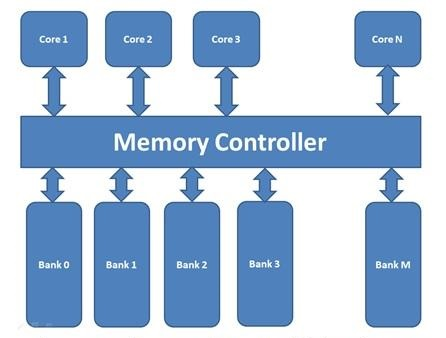
\includegraphics[width=90mm,natwidth=610,natheight=642]{multicore_arch.jpg}
\caption{Multi-core Architecture with shared memory}
\label{fig:multicore_arch}
\end{figure}
In case of multi-core processor architecture, these long-latency accesses to the shared memory encounter additional delay due to interference from accesses by the additional cores. This results in a queue of accesses waiting to be served by the memory. Figure~\ref{fig:multicore_arch}  shows a common multi-core architecture where N processor cores use a shared memory consisting of M banks. Requests from each core go to the memory controller, which then arbitrates and issues requests to the memory. Because the memory controller has parallel access to all M banks, a queue forms for each individual bank request. The queues are then served every cycle and the acknowledgement with data (in the case of a read) is sent to the processor. \\
In the scenario where multiple cores request access to the memory locations which belong to the same bank, the memory controller schedules these request for the queues of that bank. This contention between cores for memory accesses from the same bank is known as a bank conflict. When a conflict occurs, requests are served sequentially from the queues, increasing the latency for the requests later in the queue. As the number of bank conflicts increase, the latency for individual memory accesses to the same bank also increase, resulting in increased latency for the entire system. \\ 
In this report, we try to solve the problem of concentrated accesses to a particular bank by normalizing it across several banks. The problem is solved by using coding theory techniques to create redundancy across banks, increasing the number of parallel accesses per cycle. The queue build up on a bank is serviced through parallel access to several additional banks, known as parity banks. The additional bank accesses results in a decrease in number of contended memory accesses between cores, therefore reducing the overall latency of the system. The reduction in the latency can be seen directly as an increase in the overall system performance. We show that with a memory overhead of 15 $\%$; we can enable 4 extra read accesses / 2 extra write accesses to a bank while remaining within the given design parameters. 
